\documentclass[a4paper,10pt]{article}
\usepackage[utf8]{inputenc}
\usepackage[spanish]{babel}
\usepackage[pdftex]{graphicx}

\makeindex

%opening
\title{\underline{\textbf{Filesystems, IPCs y Servidores Concurrentes}}}
\author{
Lezica, Santiago. (Leg. 49147).\\
Ballesty, Pablo Andrés. (Leg. 49359).\\
Pose, Jimena Belén. (Leg. 49015).\\
}
\date{}

\begin{document}

\maketitle

\newpage
\tableofcontents

\newpage
\section{Introducción}
\subsection{Objetivo}
El objetivo de este trabajo es familiarizarse con el uso de sistemas cliente-
servidor concurrentes, implementando el servidor mediante la creación de proce-
sos hijos utilizando fork() y mediante la creación de threads. Al mismo tiempo,
ejercitar el uso de los distintos tipos de primitivas de sincronización y comunicación
de procesos (IPC) y manejar con autoridad el filesystem de Linux desde
el lado usuario.

\subsection{Enunciado}
Se desea implementar un simulador de colonia de hormigas simplificado. En
el mismo habrá un hormiguero, varias hormigas y comida esparcida a lo largo
del mundo. Las hormigas deberán recolectar la comida y traerla al hormiguero.
Para ello deberán leer la información del ambiente y comunicarse entre ellas
de manera eficiente. El objetivo de la simulación es traer la mayor cantidad
de comida al hormiguero. Después de 10000 turnos, o cuando ya no haya más
comida en el mundo, la simulación finaliza.\\
El servidor leerá del archivo de configuración la información acerca del mundo,
que tendrá forma de grilla. Particularmente estará la ubicación del hormiguero,
cada pieza de comida, su tipo (simple o grande) y las hormigas en su posición inicial.
A continuación, empezará la simulación, en donde, por turnos simultáneos, to-
das las hormigas deberán realizar una acción. Esta acción podría ser o bien:

\begin{enumerate}
 \item Moverse a un casillero contiguo horizontal o vertical.
 \item Oler los casilleros vecinos para detectar rastros, hormigas o comida.
 \item Levantar una pieza de comida que esté en un casillero contiguo horizontal o vertical.
 \item Moverse a un casillero vecino dejando un rastro.
 \item Emitir un grito.
\end{enumerate}

Dos hormigas no podrán ocupar el mismo casillero y 1 hormiga no podrá ocupar 
el mismo casillero que una pieza de comida sin levantar. En caso de que al
finalizar un turno, 2 o más hormigas intenten moverse al mismo casillero, solo
una lo logrará y la otra fallará su movimiento. La unica excepción a esta regla
es el hormiguero. Pueden haber infinitas hormigas en el casillero del hormiguero.
Las hormigas pueden dejar y detectar un rastro. Este rastro es un valor decimal
entre 0 y 1, en donde 1 es un rastro recién puesto y 0 es ”no hay rastro en
absoluto”. Al avanzar y dejar rastro, el valor de rastro dejado SIEMPRE será 
de valor 1. y por cada turno el rastro decrementará en 0.01.\\

Las hormigas SIEMPRE saben la orientación del hormiguero relativa a donde
están paradas, no así la distancia. (Es decir, una hormiga puede preguntar, sin
invertir turnos en ello, hacia donde está el hormiguero y recibir como respuesta
(N,S,E,W,NE,NW,SE,SW).\\

Las hormigas tienen una memoria muy limitada y solo pueden recordar 2 posiciones 
en el mapa, una de ellas siendo siempre el hormiguero. Es decir, una
hormiga puede decidir almacenar una posición del tablero para luego preguntarse
en que dirección está.\\

Las hormigas tienen una memoria muy limitada y solo pueden recordar 2 posiciones 
en el mapa, una de ellas siendo siempre el hormiguero. Es decir, una
hormiga puede decidir almacenar una posición del tablero para luego preguntarse
en que dirección está.
Cuando una hormiga grita, todas las hormigas reciben la posición de la hormiga
que grita y la distancia hamiltoniana entre ellas. Al escuchar un grito, una
hormiga puede optar por reemplazar su memoria por la posición de la hormiga
que gritó.\\

Existen 2 tipos de comida: chica y grande. La comida chica puede ser transportada 
por una hormiga sin dificultad y tiene valor 1. La hormiga simplemente
tiene que posicionarse en un casillero contiguo y utilizar un turno para levantar
la comida. La comida grande vale 5 puntos, puede ser transportada por una
hormiga, pero necesita de 2 hormigas para ser levantada, es decir: debe haber
2 hormigas posicionadas contigua a la comida y ambas deben utilizar un turno
para levantar o asistir en levantar la comida.\\

\subsection{Actividades}
Implemente la simulación utilizando procesos y threads y haga cuatro versiones del sistema, 
usando las siguientes primitivas de IPC:
\begin{enumerate}
 \item 
    \begin{itemize}
      \item Pipes o fifos.
      \item Colas de mensajes - System V o POSIX.
      \item Memoria compartida o mmap(), Semáforos System V o POSIX.
      \item Sockets - TCP o de dominio Unix.
    \end{itemize}
  \item El archivo de configuración tendrá el siguiente formato:
    \begin{itemize}
     \item Una línea con la longitud y alto del tablero separados por coma. Ej: 6,8
      significa un tablero de 6 columnas y 8 filas.
     \item Una línea con la posición del hormiguero separada por coma, teniendo en
      cuenta que la posición superior izquierda es 0,0. Ej: 3,4 significa que el
      hormiguero está en la cuarta columna, quinta fila.
     \item Una línea con la cantidad de hormigas N. Todas las hormigas empiezan
      en el hormiguero.
     \item Una línea con la cantidad de comida chica M, seguida de M líneas con la
      posición de cada comida.
     \item Una línea con la cantidad de comida grande K, seguida de K líneas con la
      posición de cada comida.
    \end{itemize}
  \item El programa debe permitir la visualización de la simulación en un tablero en
   la pantalla, iterando turno a turno.
  \item Todas las hormigas deben tener la misma programación, es decir, si bien
  lo que hacen dependerá de su posición y pueden elegir moverse a un lugar al
  azar, debe haber una unica función con la programación para todas las hormigas
  individuales.
  \item La nota del trabajo prático no dependerá de la eficiencia de la simulación,
   sin embargo, la cátedra proveerá 3 escenarios de prueba y se otorgará un punto
    extra al equipo que maximice puntajes en estos 3 escenarios.

\end{enumerate}

\newpage

\section{Desarrollo}
\subsection{Modelado del problema}
Para el desarrollo de la simulación de hormigas decidimos modelar a cada hormiga como un proceso, el cual dispara un \textit{thread} que se
encarga de la comunicación de esta hormiga con el \textit{server}. De la misma manera, el \textit{server} es un proceso que dispara un thread
que se encarga de la comunicación de éste con las hormigas de este mini-universo.\\
Los \textit{threads} aprovechando que comparten los datos con el proceso que los dispara, se encargarán de recibir y enviar constantemente los 
mensajes entrantes y salientes, a través de los distintos sistemas de \textbf{IPC}, estos mensajes entrantes y salientes serán debidamente
encolados o desencolados de las colas \textit{inbox} y \textit{outbox} que posee cada proceso en ejecución.\\
A continución se coloca una ilustración de un server conectado con dos hormigas:

\begin{center}
 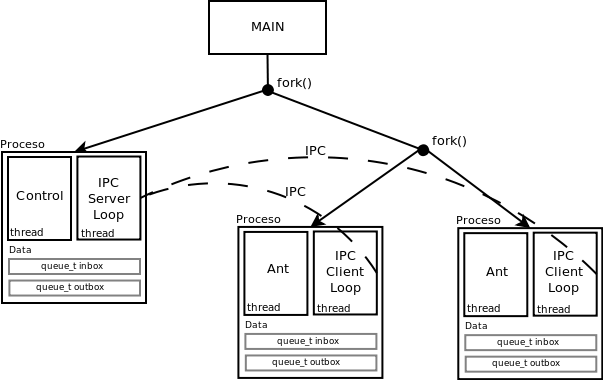
\includegraphics[scale=0.65]{./so1.png}
 % so1.png: 603x380 pixel, 72dpi, 21.27x13.41 cm, bb=0 0 603 380
\end{center}

\subsection{Implementación de IPCs}
\subsubsection{Fifos}
Para entablar una comunicación entre procesos mediante el sistema de IPC implementado con \textbf{FIFOS}, se tomaron las siguientes decisiones:
\begin{itemize}
 \item Al iniciar el proceso \textit{server} creará en el directorio ``/tmp'', todas las fifos necesarias para entablar comunicación 
con las \textit{n} hormigas participantes.
 \item Los nombres de cada fifo corresponden a la siguiente regla: La hormiga con id lógico \textit{n} enviará mensajes a través de la fifo 
``\verb|/tmp/fifo_c_w_n|'' y recibirá mensajes a través de la fifo ``\verb|/tmp/fifo_c_r_n|''. De esta manera entabla una comunicación
bidireccional con el \textit{server}.
  \item Se asume que en el directorio ``/tmp'' no hay fifos creadas con los mismos nombres, el programa se asegura crear y eliminar todas las 
fifos utilizadas.

\subsubsection{Memoria compartida y semáforos}
Para la implementación del IPC con \textbf{Memoria compartida} se utilizó la propuesta de \textbf{System V} para allocar memoria compartida, y 
2 semáforos binarios o locks.
Se crearon dos buffers circulares, en uno el proceso \textit{server} escribe los mensajes para los clientes y en el otro lee los mensajes que
le envían. En cada acceso a cada buffer, se utiliza un lock para evitar problemas de sincronización.\\
A su vez cada cliente, lee del buffer donde el server escribe, y escribe en el buffer de donde lee el server, siempre lockeando en los accesos.
De esta manera se logra una comunicación bidireccional entre un proceso cliente y un proceso server.
\end{itemize}






\bigskip
\end{document}
